
\begin{theo}[Chapter Reference]{thm:pythagoras}
  The contents of the chapter is based on:
  \vspace{-0.4cm}
  \begin{itemize}
    \item Bayoumi, M., Nomidis, S. K., Willems, K., Carlon, E., and Maglia, G. (2021).
      Autonomous and active transport operated by an entropic DNA piston.\\
      Nano Letters, 21(1):762–768. PMID: 33342212.
  \end{itemize}
  \vspace{0.3cm}
\end{theo}

Recently, a DNA nanopiston based molecular machine has been developed by the Maglia
research group. Its main function constitutes the turning over of chemical fuel, in the
form of ssDNA, into autonomous and active transport. The design is based upon the group's
earlier work, where they developed a protein rotaxane \cite{Biesemans2015}, consisting of
a polypeptide thread trapped in
a ClyA nanopore by two stopper proteins. This rotaxane could be moved between two stable
states inside the nanopore using an electric potential, acting as a molecular switch.

Motivated by the results from this research, the DNA nanopiston was developed by Bayoumi
et al. In this new molecular machine the rotaxane constitutes of
a DNA strand instead of a polypeptide thread. Utilising the thermodynamic transitions of
DNA, this complex is capable of actively transporting DNA cargo-strands through the
nanopore.

In this chapter the work of Bayoumi et al. is discussed, giving an overview of the
construction and operating cycle of this molecular machine.  At the end of this chapter
the molecular dynamics simulations from the paper of Bayoumi et al. are discussed, as
they where the main inspiration behind our project.

\section{Rotaxane Formation}

Synthetic molecular machines are often times embedded in larger complexes, providing the
necessary structure for their operation. For this reason biological nanopores are a
suitable starting point in the development of molecular machines. These transmembrane
proteins spontaneously self-assemble into well-defined structures, embedded into a lipid
bilayer. Extensive research has been performed towards designing methods and tools to
tailor their structural and electrostatic properties for specific use cases, originally
focused on ionic current spectroscopy. This large back catalogue of research can now be
employed into building out their utility as an ideal building block for membrane bound
molecular machines.

The design of the DNA nanopiston is centered around the biological nanopore Cytolysin
A (ClyA). A modified variant ClyA-AS is used, which has been specially engineered for
use in ionic current spectroscopy.\cite{Soskine2012} By virtue of the large inner lumen
of ClyA,
translocation of dsDNA through the pore is possible. The molecular machine utilises this
property by capturing a DNA rotaxane structure inside of the pore, anchoring it to the
lipid membrane. The rotaxane is composed of a DNA complex connected to two neutravidin
protein stoppers via biotin, which serves to keep the structure captured in the pore.
The bioton vitamin strongly binds to avidin proteins, resulting in a very stable
connection, an often used tool in biotechnology. The DNA complex consists of three single
stranded DNA's:  ssDNA $1$, ssDNA $2$, and ssDNA $3$, as shown in Figure
\ref{fig:formation}a.

Formation of the DNA nanopiston takes place in a saline filled reservoir, where a
ClyA nanopore is embedded into a membrane partitioning the reservoir into a cis- and
trans-side. To start the formation process neutravidin ($0.5\ \mu M$), ssDNA $1$
($5′-\text{biotinylated, }100\text{ nt, }1.2\ \mu M$) and ssDNA $2$ ($80\text{ nt, }1
\mu M$) are added to the cis-compartment. Since the first $70$ nucleotides of ssDNA $1$
are complementary to the last $70$ nucleotides of ssDNA $2$, the two strands will
partially hybridise. This results in a DNA duplex structure with on one side two ssDNA
overhangs and on the other side a neutravidin stopper, as shown in (ii) of Figure
\ref{fig:formation}b.

Applying a voltage of $+100\ mV$ over the reservoir results in a net force guiding the
DNA complex from the cis-side towards the trans-side. The applied potential drives the
capturing of the DNA inside the nanopore, observed as a drop in the pore current, see
Figure \ref{fig:formation}c. The complex remains indefinitely captured inside until the
applied potential is reversed, restoring the open-pore current.

Finally, neutravidin ($1\ \mu M$) and ssDNA $3$ ($3\text{′-biotinylated, }20\text{ nt, }2
\mu\ M$) are brought into the solution at the trans-side, while keeping the potential at
$+ 100\ mV$. The longest overhang of the captured DNA thread is formed by the 30 free
nucleotides of ssDNA $1$. The added strand, ssDNA $3$, is fully complementary with the
last $20$ nucleotides of this overhang, resulting in the hybridisation of both strands,
shown in (iii) of Figure \ref{fig:formation}b.

To verify if the hybridisation has successfully taken place, the voltage over the
reservoir is reversed. If no difference is measured in the pore-current, we conclude that
the stable structure is formed, capturing the rotaxane inside the pore by the two protein
stoppers. After the hybridisation we find the final structure, which is referred to as
the rotaxane-ds.

\begin{figure}[h!]
  \begin{centering}
  \adjustbox{minipage=1.3em,valign=t}{\subcaption{}\label{sfig:testa}}%
  \begin{subfigure}[t]{\dimexpr0.93\linewidth-1.3em\relax}
  \centering
  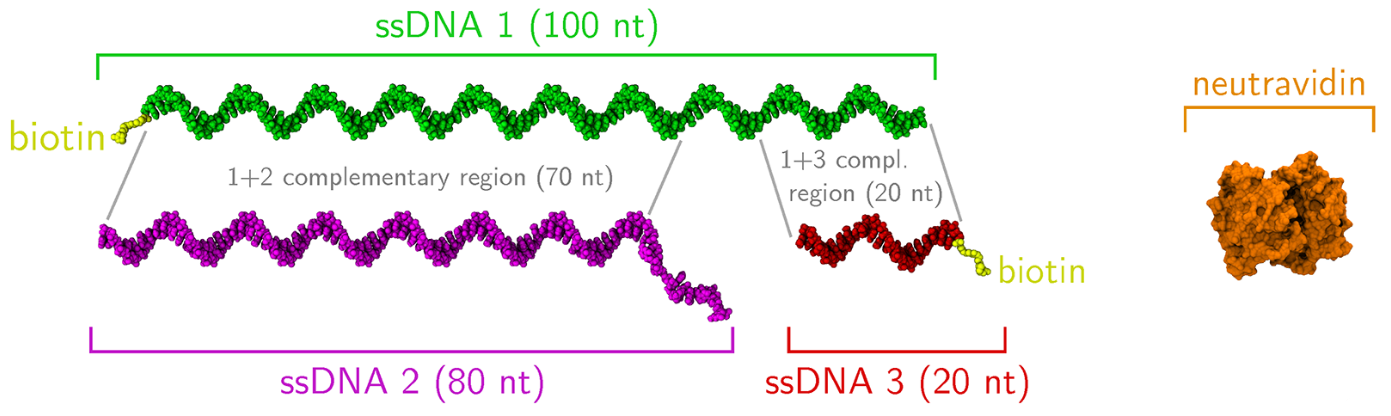
\includegraphics[width=\linewidth,valign=t]{Figures/RConstruction1.png}
  \end{subfigure}%
  \vspace{0.2cm}
  \adjustbox{minipage=1.3em,valign=t}{\subcaption{}\label{sfig:testa}}%
  \begin{subfigure}[t]{\dimexpr0.93\linewidth-1.3em\relax}
  \centering
  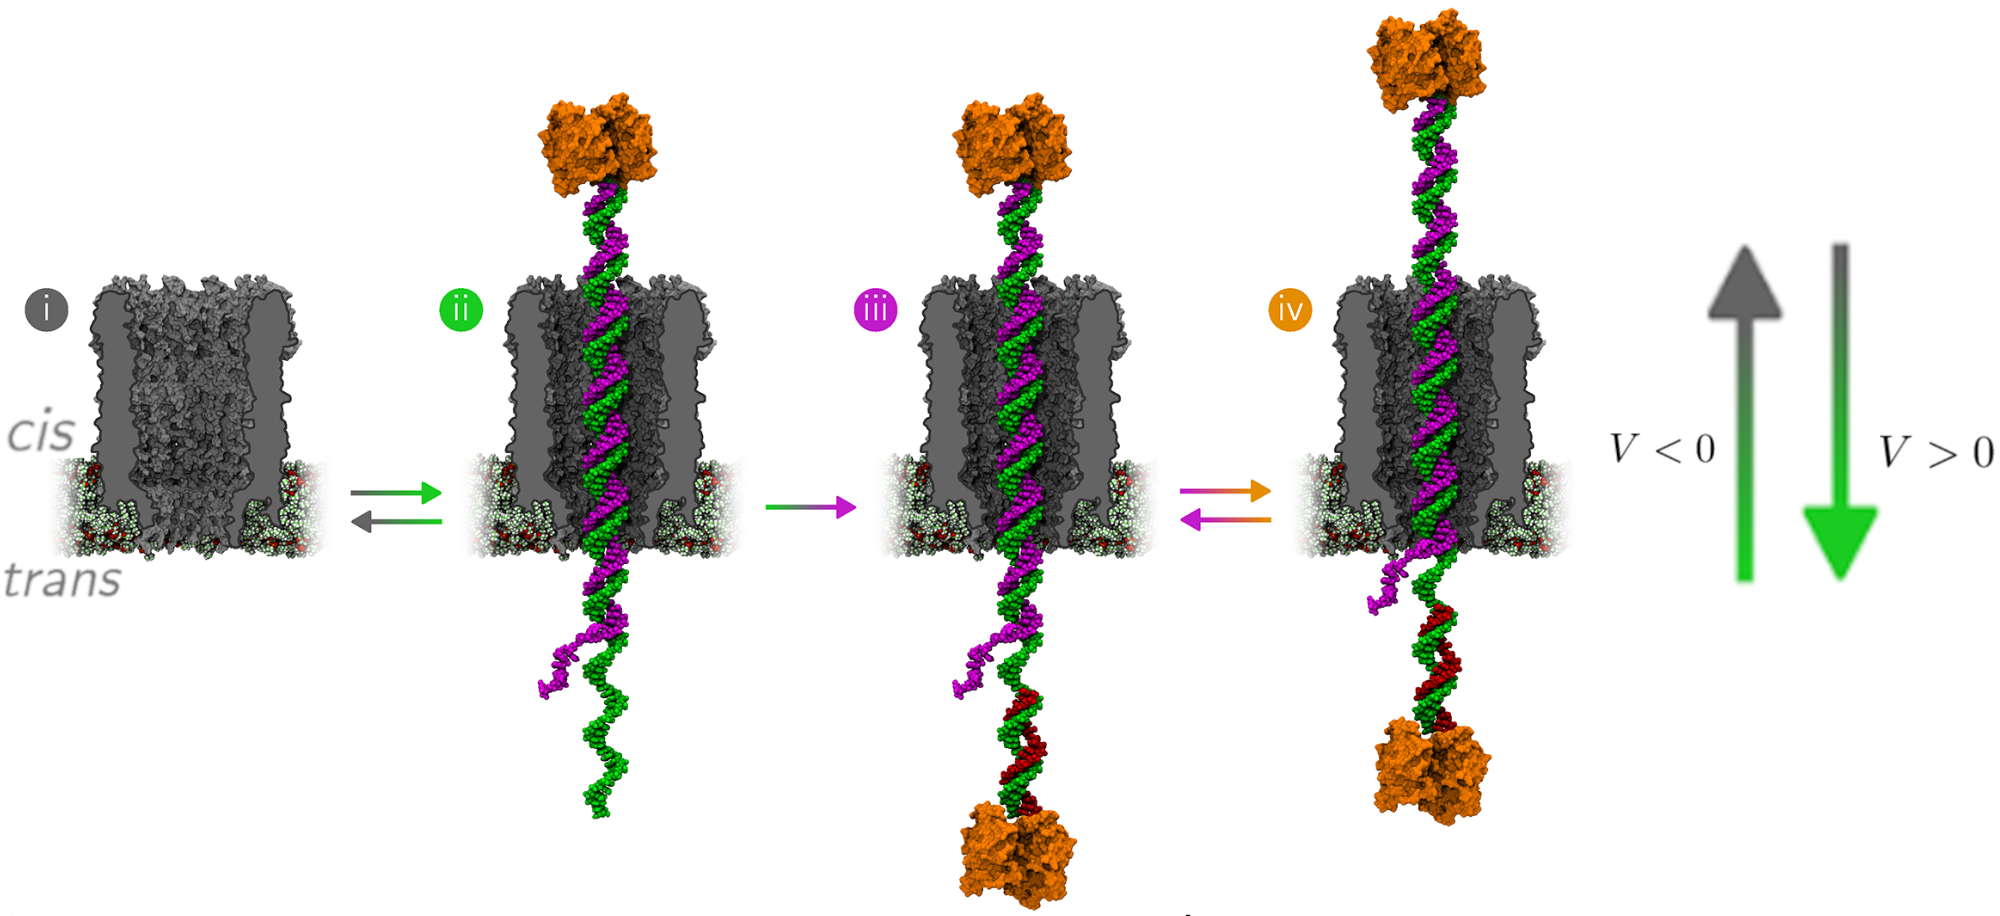
\includegraphics[width=\linewidth,valign=t]{Figures/RConstruction4.png}
  \end{subfigure}%
  \vspace{0.2cm}
  \adjustbox{minipage=1.3em,valign=t}{\subcaption{}\label{sfig:testb}}%
  \begin{subfigure}[t]{\dimexpr0.93\linewidth-1.3em\relax}
  \centering
  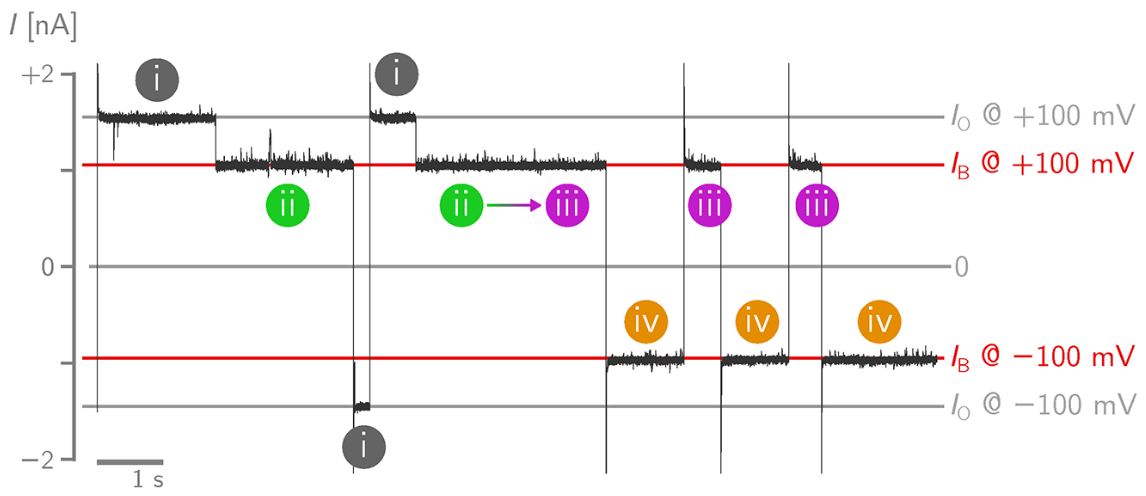
\includegraphics[width=\linewidth,valign=t]{Figures/RConstruction3.png}
  \end{subfigure}
  \caption[Illustrations of the DNA nanopiston formation.]{\linespread{0.1}{\small
  Illustrations of the DNA nanopiston formation process. (a) The individual components
  making up the rotaxane-ds. The different DNA strands with
  their complementary regions are shown alongside the neutravidin molecule. (b) Snapshots
  of the assembly process of rotaxane-ds. The arrows on the right indicate the direction
  of the induced force by an applied potential. (c) The corresponding current traces
  measured during the assembly process are plotted. Labels in (a) and (b) relate the
  measured current with a specific intermediate state of the assembly process. Images
  adapted from reference \cite{Bayoumi21}.}}
  \label{fig:formation}
  \end{centering}
\end{figure}
